\documentclass{beamer}
\usepackage[utf8]{inputenc}

\mode<presentation>{
	\usetheme{AnnArbor}
	\usecolortheme{crane}
}
\title{The Lazy Man's Cycle Starter}
\subtitle{Presentation on the Box2D project of Group 14}
\author{
	C Vishwesh \\
   \texttt{Roll No. 140050031}\\
\and
	Saurabh Garg \\
   \texttt{Roll No. 140070003}\\
%    saurabhgarg@cse.iitb.ac.in}\\
\and
	Aviral Kumar \\
	\texttt{Roll No. 140070031}
%	aviral@cse.iitb.ac.in}\\
}
\date{October 19, 2015}
\begin{document}
\begin{frame}
	\titlepage
\end{frame}
\begin{frame}
\frametitle{Overview}
	\tableofcontents[
		%sectionstyle=show/shaded,
	]
\end{frame}
\section{Introduction}
\begin{frame}
\setbeamercovered{transparent}
	\frametitle{Introduction}
	\begin{enumerate}
	 \item \onslide<1->{This is a project where a Rube Goldberg machine has been simulated in the Physics Game Engine, Box2D}
	 \item	\onslide<2->{Aim is to make a man stuck on a cycle with square wheels on a road made of Catenary curves move without doing any considerable work.}
	 \item \onslide<3->{The man pulls a rope hanging in front of him, and thus triggers a chain reaction which finally gives him the impulse to move}
	 \item \onslide<4->{Elements used in this simulation include : Spirals, Catenary curves, spring mass system, two pulley system, Bicycle, Hourglass and some other common elements.}
	\end{enumerate}
\end{frame}
\section{Technical Details}
\subsection{Components}
\begin{frame}
\setbeamercovered{transparent}
\frametitle{Components}
\begin{columns}
\column{0.55\textwidth}
\begin{enumerate}
\item \onslide<1-> \textbf{Helix} : This is a helix shaped or a spiral path where the ball can move. It has been made using a box2d chain object by joining the points obtained from the mathematcial equation of the curve.
\item \onslide<2-> \textbf{Catenary curves} : These are special curves such that a properly oriented square can move on them smoothly. The mathematical equation is: 
$y = cosh(\frac{x}{a})$
\end{enumerate}
\column{0.45\textwidth}
\center{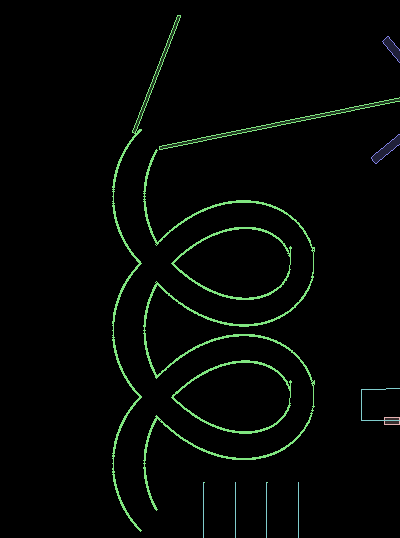
\includegraphics[scale=0.19]{helix.png}}\\ 
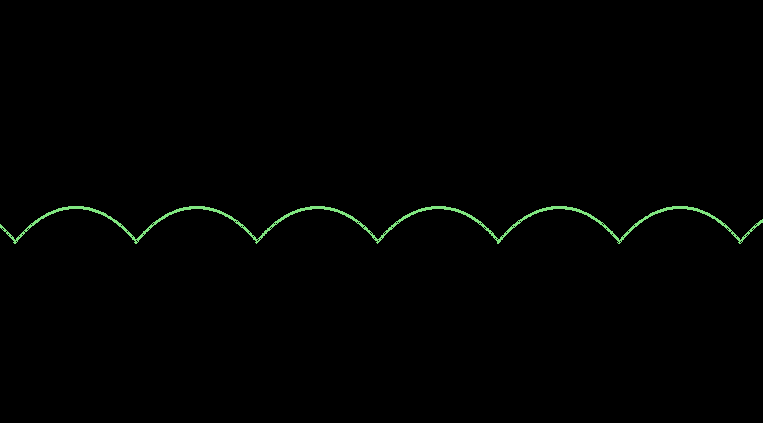
\includegraphics[scale=0.15]{catenary2.png}
\end{columns}
\end{frame}

\begin{frame}
\setbeamercovered{transparent}
\frametitle{Components...}
\begin{columns}
\column{0.55\textwidth}
\begin{enumerate}
\item \onslide<1-> \textbf{Two Pulley system} : This is a complex pulley system which looks relatively simpler. Two pulley joints share a common rope (edge). This has been made by making an object common to both the pulleys and asetting its gravity to be zero.
\item \onslide<2-> \textbf{Spring Mass system} : This system comprises of two bodies connected by an elastic string which beahves like a spring and gives effects like extension, compression, etc.  
\end{enumerate}
\column{0.45\textwidth}
\center{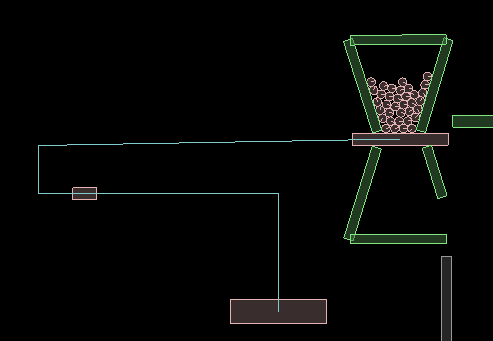
\includegraphics[scale=0.20]{2pulley.png}}\\
\center{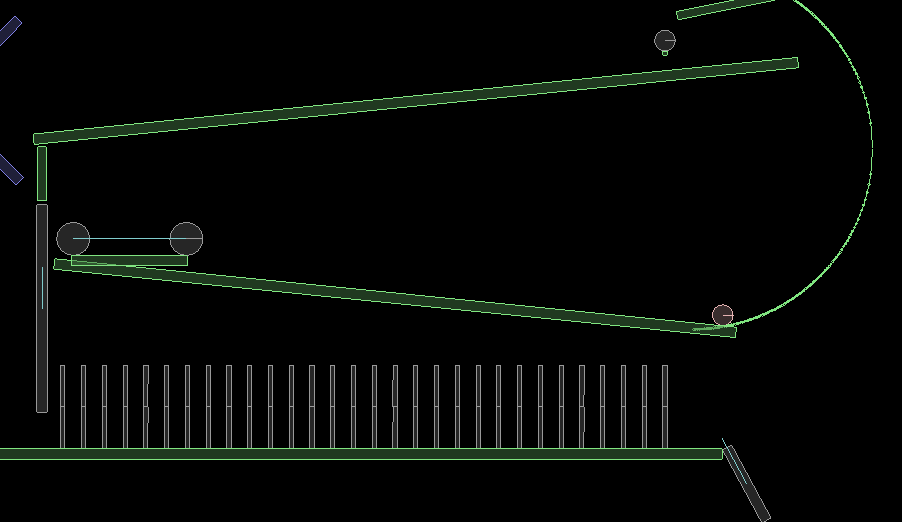
\includegraphics[scale=0.17]{springmass.png}}
\end{columns}
\end{frame}
\subsection{Working}
\begin{frame}
\setbeamercovered{transparent}
\frametitle{Working in brief}
\begin{enumerate}
\item \onslide<1-> The man sitting on the cycle pulls the rope hanging in front of him downwards (this has ben implemented by providing the user the chance to pull the rope down) which triggers a chain reaction.
\item \onslide<2-> The balloon gets freed and moves up, hits the rod connected by a hinge to the plank on which the dominos are kept. This rod hits the dominos which fall down one by one. 
\item \onslide<3-> Energy is transfered to the left end and then to the spring mass system, which hits a ball which starts moving up after that and hits another ball at the top.
\item \onslide<4-> This ball crosses over the fans/ turbines and enter the spiral helix path, finally leaving it and hitting the Newon's pendulum, which hits the cycle and brings it into motion.
\end{enumerate}

\end{frame}
\subsection{Screenshot}
\begin{frame}
\center{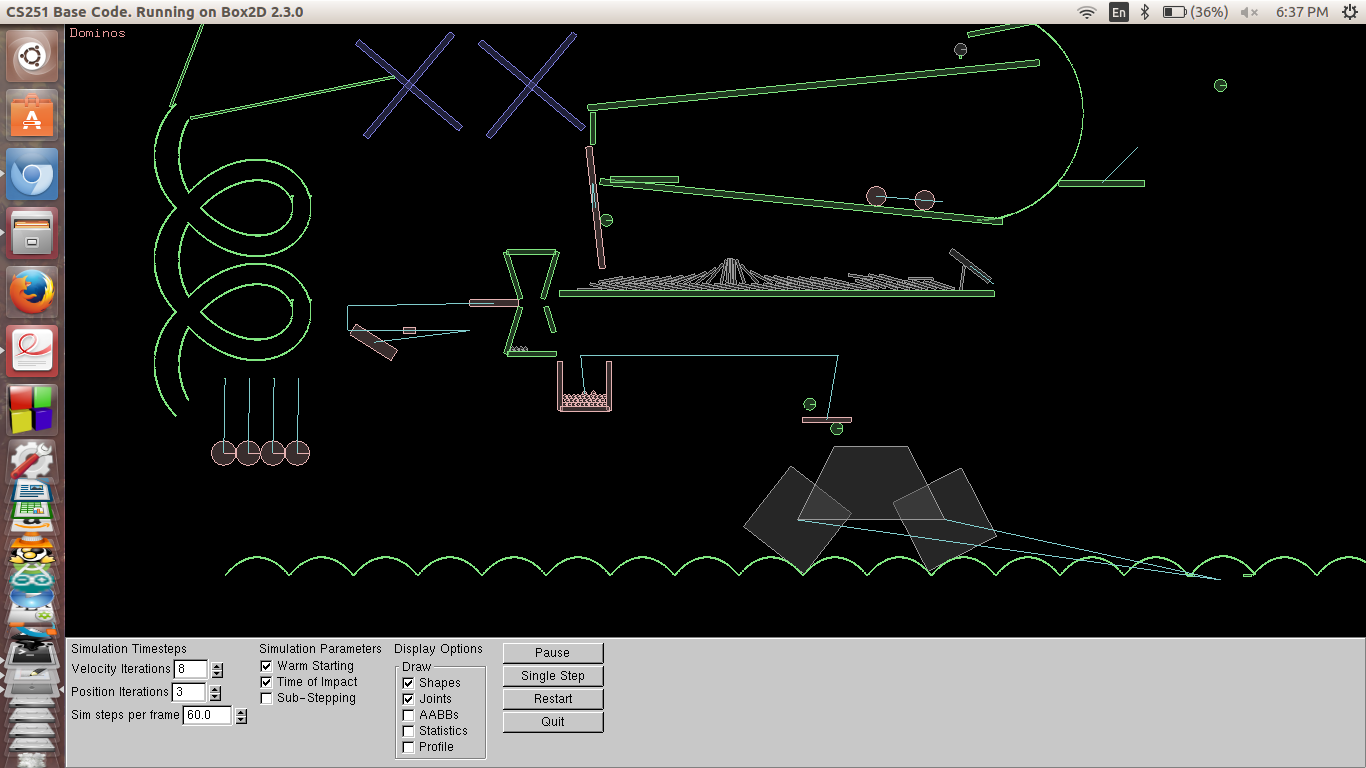
\includegraphics[scale=0.24]{screenshot.png}}
\end{frame} 

\section{Conclusion}
\begin{frame}
\frametitle{Conclusion}
%\begin{enumerate}
The project was quite interesting. It gave us an exposure to programming in a game engine like Box2D in a basic language like C++ which we alredy knew. Making the project was a job that we enjoyed a lot. We look forward to getting such opportunities furthur ahead.\\
\center{THANK YOU!} 
%\end{enumerate}
\end{frame}
\end{document}
